\documentclass[12pt,a4paper]{article}
\usepackage[utf8]{inputenc}
\usepackage{array}
\usepackage{geometry}
\usepackage{graphicx}
\usepackage{fancyhdr}
\usepackage{amsmath}
\usepackage{amsfonts}
\usepackage{amssymb}
\usepackage{color}
\usepackage{hyperref}
\usepackage{listings}
\usepackage{tikz}
\usetikzlibrary{shapes.geometric,arrows,positioning,shadows}
\usepackage{pgfgantt}
\usepackage{float}
\usepackage{xcolor}
\usepackage{booktabs}
\usepackage{multirow}
\usepackage{subcaption}
\usepackage{titlesec}
\usepackage{multicol}
\usepackage{caption}
\usepackage{colortbl}

% ===================== PROFESSIONAL COLOR SCHEME =====================
% Define professional color palette
\definecolor{primaryblue}{RGB}{0,82,165}        % Deep professional blue
\definecolor{secondaryblue}{RGB}{25,118,210}    % Medium blue
\definecolor{accentblue}{RGB}{100,181,246}      % Light blue accent
\definecolor{lightblue}{RGB}{173,216,230}       % Light blue for backgrounds
\definecolor{darkgray}{RGB}{66,66,66}           % Professional dark gray
\definecolor{mediumgray}{RGB}{117,117,117}      % Medium gray
\definecolor{lightgray}{RGB}{238,238,238}       % Light gray for backgrounds

% Professional table formatting with coordinated styling
\definecolor{tableheader}{RGB}{0,82,165}         % Primary blue for headers
\definecolor{tablebody}{RGB}{240,248,255}        % Very light blue
\definecolor{tableaccent}{RGB}{25,118,210}       % Secondary blue accent
\definecolor{tableborder}{RGB}{0,82,165}         % Primary blue border

% Additional color definitions for enhanced tables
\definecolor{headertext}{RGB}{255,255,255}       % White text for headers
\definecolor{bodytext}{RGB}{66,66,66}            % Professional dark gray
\definecolor{tablealt1}{RGB}{248,251,255}        % Alternating row color 1
\definecolor{tablealt2}{RGB}{235,245,251}        % Alternating row color 2
\definecolor{greentable}{RGB}{76,175,80}         % Professional green
\definecolor{orangetable}{RGB}{255,152,0}        % Professional orange
\definecolor{purpletable}{RGB}{156,39,176}       % Professional purple

% Enhanced table styling commands
\newcommand{\tableheaderrow}[1]{\rowcolor{tableheader}\textcolor{headertext}{\textbf{#1}}}
\newcommand{\tablealtrow}{\rowcolor{tablealt1}}
\newcommand{\tablealtrowtwo}{\rowcolor{tablealt2}}
\newcommand{\specialheader}[2]{\rowcolor{#1}\textcolor{headertext}{\textbf{#2}}}

% Set default array rule width for professional borders
\setlength{\arrayrulewidth}{1.2pt}

% Professional caption configuration - coordinated styling
\captionsetup{
    font={bf,small},
    textfont={color=bodytext},
    labelfont={color=primaryblue, bf},
    justification=centering,
    singlelinecheck=false,
    labelsep=period,
    skip=10pt,
    position=bottom
}

% Professional subcaption formatting - coordinated styling
\captionsetup[sub]{
    font={bf,footnotesize},
    textfont={color=bodytext},
    labelfont={color=secondaryblue, bf},
    justification=centering,
    singlelinecheck=false,
    labelsep=period,
    skip=8pt
}

% Configure hyperref with professional colors
\hypersetup{
    colorlinks=true,
    linkcolor=primaryblue,
    filecolor=secondaryblue,      
    urlcolor=accentblue,
    pdftitle={Lab 5: Iris Dataset Classification Analysis},
    pdfauthor={Sajidur Rahman Tarafder},
    pdfsubject={Data Mining Lab Report - Iris Classification}
}

% Enhanced code listings with professional colors
\lstset{
    basicstyle=\ttfamily\footnotesize,
    backgroundcolor=\color{lightgray},
    frame=leftline,
    framerule=3pt,
    rulecolor=\color{primaryblue},
    breaklines=true,
    captionpos=b,
    numbers=left,
    numberstyle=\tiny\color{darkgray}\bfseries,
    stepnumber=1,
    numbersep=12pt,
    keywordstyle=\color{primaryblue}\bfseries,
    commentstyle=\color{mediumgray}\itshape,
    stringstyle=\color{secondaryblue},
    emphstyle=\color{accentblue}\bfseries,
    showstringspaces=false,
    tabsize=2,
    xleftmargin=20pt,
    framexleftmargin=15pt,
    numberbychapter=false,
    firstnumber=1
}

% Professional section formatting with modern styling
\titleformat{\section}[hang]
{\normalfont\LARGE\bfseries\color{primaryblue}}
{\colorbox{primaryblue}{\makebox[1.8em]{\textcolor{white}{\thesection}}}~}{0.5em}
{}
[\vspace{2pt}{\color{primaryblue}\hrule height 1pt width \textwidth}]
\titlespacing*{\section}{0pt}{25pt}{18pt}

% Professional subsection formatting with perfect left alignment
\titleformat{\subsection}[block]
{\normalfont\Large\bfseries\color{secondaryblue}}
{\thesubsection.~}{0pt}
{}
[\vspace{1pt}{\color{secondaryblue}\hrule height 0.8pt width \textwidth}]
\titlespacing*{\subsection}{0pt}{20pt}{14pt}

% Modern subsubsection formatting with perfect left alignment
\titleformat{\subsubsection}[block]
{\normalfont\large\bfseries\color{accentblue}}
{\thesubsubsection.~}{0pt}
{}
[\vspace{0.5pt}{\color{accentblue}\hrule height 0.5pt width \textwidth}]
\titlespacing*{\subsubsection}{0pt}{15pt}{10pt}

% Define custom project title formatting (left-aligned with consistent underlines)
\newcommand{\projecttitle}[1]{
    \vspace{12pt}
    {\normalfont\large\bfseries\color{accentblue}#1}
    \vspace{0.5pt}
    {\color{accentblue}\hrule height 0.5pt width \textwidth}
    \vspace{8pt}
}

% Professional geometry settings for maximum content utilization
\geometry{
    a4paper,
    left=2.5cm,
    right=2.5cm,
    top=3cm,
    bottom=3cm,
    headheight=25pt,
    headsep=30pt,
    footskip=30pt,
    includeheadfoot
}

% Enhanced header and footer styling
\pagestyle{fancy}
\fancyhf{}
\fancyhead[L]{\textcolor{primaryblue}{\textbf{Lab Report}}}
\fancyhead[R]{\textcolor{secondaryblue}{\textbf{CSE 4120 - Data Mining Sessional}}}
\fancyfoot[C]{\textcolor{darkgray}{\thepage}}
% Footer setup - only page number
\fancyfoot[C]{\textcolor{primaryblue}{\textbf{\thepage}}}
    
% No footer line
\renewcommand{\footrulewidth}{0pt}
\renewcommand{\headrulewidth}{2pt}
\renewcommand{\footrulewidth}{1pt}
\renewcommand{\headrule}{\hbox to\headwidth{%
    \color{primaryblue}\leaders\hrule height \headrulewidth\hfill}}
\renewcommand{\footrule}{\hbox to\headwidth{%
    \color{lightgray}\leaders\hrule height \footrulewidth\hfill}}

\begin{document}

% ===================== COVER PAGE =====================

\begin{titlepage}
    \thispagestyle{empty}
    \centering
    
    % University motto
    {\large \textbf{"Heaven's Light is Our Guide"}}\\[0.3cm]
    
    % University logo
    \includegraphics[width=4cm]{ruet_logo.png} \\[0.4cm]
    
    % University name
    {\Large \textbf{Department of Computer Science \& Engineering}}\\[0.3cm]
    {\large \textbf{Rajshahi University of Engineering \& Technology}}\\[0.8cm]

    \vspace{0.8cm}
    % Report title
    {\LARGE \textbf{Lab Report}}\\[0.4cm]

    \vspace{0.5cm}
    % Course details
    {\Large \textbf{Course Code: CSE 4120}}\\[0.3cm]
    {\Large \textbf{Course Title: Data Mining Sessional}}\\[0.4cm]
    
    
    % Submission details table with proper formatting
    \begin{table}[h!]
    \centering
    \setlength{\arrayrulewidth}{1.5pt}
    \renewcommand{\arraystretch}{1.5}
    \begin{tabular}{|p{8.5cm}|p{6.5cm}|}
        \hline
        \multicolumn{1}{|c|}{\large \textbf{Submitted By:}} & \multicolumn{1}{c|}{\large \textbf{Submitted To:}} \\
        \hline
        & \\
        \large \textbf{Name: Sajidur Rahman Tarafder} & \multirow{5}{*}{\parbox{6.5cm}{\centering 
        \large \textbf{Julia Rahman} \\ 
        \vspace{0.2cm}
        \large \textbf{Associate Professor} \\ 
        \vspace{0.2cm}
        \large \textbf{Department of CSE RUET} \\ 
        \vspace{0.4cm}}} \\
        \large \textbf{Roll: 2003154} & \\
        \large \textbf{Section: C} & \\
        \large \textbf{Session: 2020-21} & \\
        \large \textbf{Department: CSE} & \\
        & \\
        \hline
    \end{tabular}
    \end{table}
    
    \vspace{0.5cm}
\end{titlepage}

% ===================== TABLE OF CONTENTS =====================
\newpage
\thispagestyle{fancy}
\tableofcontents
\newpage

% ===================== INTRODUCTION =====================
\section{ Lab-5: Classification Analysis }

\subsection{Introduction}
The Iris dataset represents an ideal learning platform for classification algorithms due to its balanced structure, clear feature relationships, and well-defined class boundaries. Through systematic implementation of both Decision Trees and Na\"{i}ve Bayes approaches, this study provides valuable insights into the comparative effectiveness of rule-based versus probabilistic classification methodologies.

\subsection{Objective}
The primary objective of this laboratory session is to develop practical expertise in supervised classification techniques through hands-on implementation and rigorous evaluation. This work encompasses dataset preparation, algorithm implementation, model training and testing, performance evaluation using cross-validation techniques, and comprehensive analysis of classification results including confusion matrix interpretation and precision-recall metrics assessment.
\section{Dataset Characteristics}

The Fisher's Iris dataset contains 150 carefully collected samples representing three distinct species of iris flowers: Iris Setosa, Iris Versicolor, and Iris Virginica. Each sample is characterized by four morphological measurements: sepal length, sepal width, petal length, and petal width, all recorded in centimeters with high precision.

This dataset exhibits several characteristics that make it particularly suitable for classification analysis: perfectly balanced class distribution with exactly 50 samples per species, continuous numerical features with clear discriminative patterns, minimal missing values or data quality issues, and well-established ground truth labels that enable reliable performance assessment.

The morphological features demonstrate varying degrees of discriminative power across the three iris species. Sepal and petal measurements provide complementary information about flower structure, with certain features showing stronger correlation with specific species classifications. This natural feature diversity allows for comprehensive evaluation of algorithm performance under different classification scenarios.

% ===================== CLASSIFICATION USING DECISION TREES =====================
\section{Classification using Decision Trees}

\subsection{Dataset Loading and Preparation}

\subsubsection{Implementation Approach}
I loaded the Iris dataset using pandas to read the CSV file and prepared it for classification analysis. My approach involved importing essential libraries like pandas for data handling, numpy for numerical operations, matplotlib for visualization, and sklearn for machine learning tasks. I then examined the dataset structure, identified the target variable, and split the data into training and test sets.

\subsubsection{Implementation Code}
\begin{lstlisting}[language=Python, caption=Dataset Loading and Data Preparation]
# Importing necessary libraries
import pandas as pd
import numpy as np
import matplotlib.pyplot as plt
from sklearn.model_selection import train_test_split, cross_val_score
from sklearn.tree import DecisionTreeClassifier, plot_tree
from sklearn.naive_bayes import GaussianNB
from sklearn.metrics import accuracy_score, confusion_matrix, precision_score, recall_score

print("Libraries imported successfully!")

# Loading the dataset
df = pd.read_csv('iris.csv')
print("Loaded iris.csv successfully!")

# Checking data dimensions and types
print(f"Dataset dimensions: {df.shape}")
print(f"Columns: {df.columns.tolist()}")
print(f"Data types:")
print(df.dtypes)

# Potential label columns
print("First few rows:")
print(df.head())
print(f"\nPotential label column: {df.columns[-1]}")
print(f"Unique values in label: {df[df.columns[-1]].unique()}")

# Preparing features and target variable
X = df.drop('variety', axis=1)
y = df['variety']

# Splitting data into training and test sets (80-20)
X_train, X_test, y_train, y_test = train_test_split(X, y, test_size=0.2, random_state=42, stratify=y)

print(f"Training set: {X_train.shape[0]} samples")
print(f"Test set: {X_test.shape[0]} samples")
print(f"Features: {X.columns.tolist()}")
\end{lstlisting}

\subsubsection{Terminal Output}
\begin{figure}[h!]
\centering
    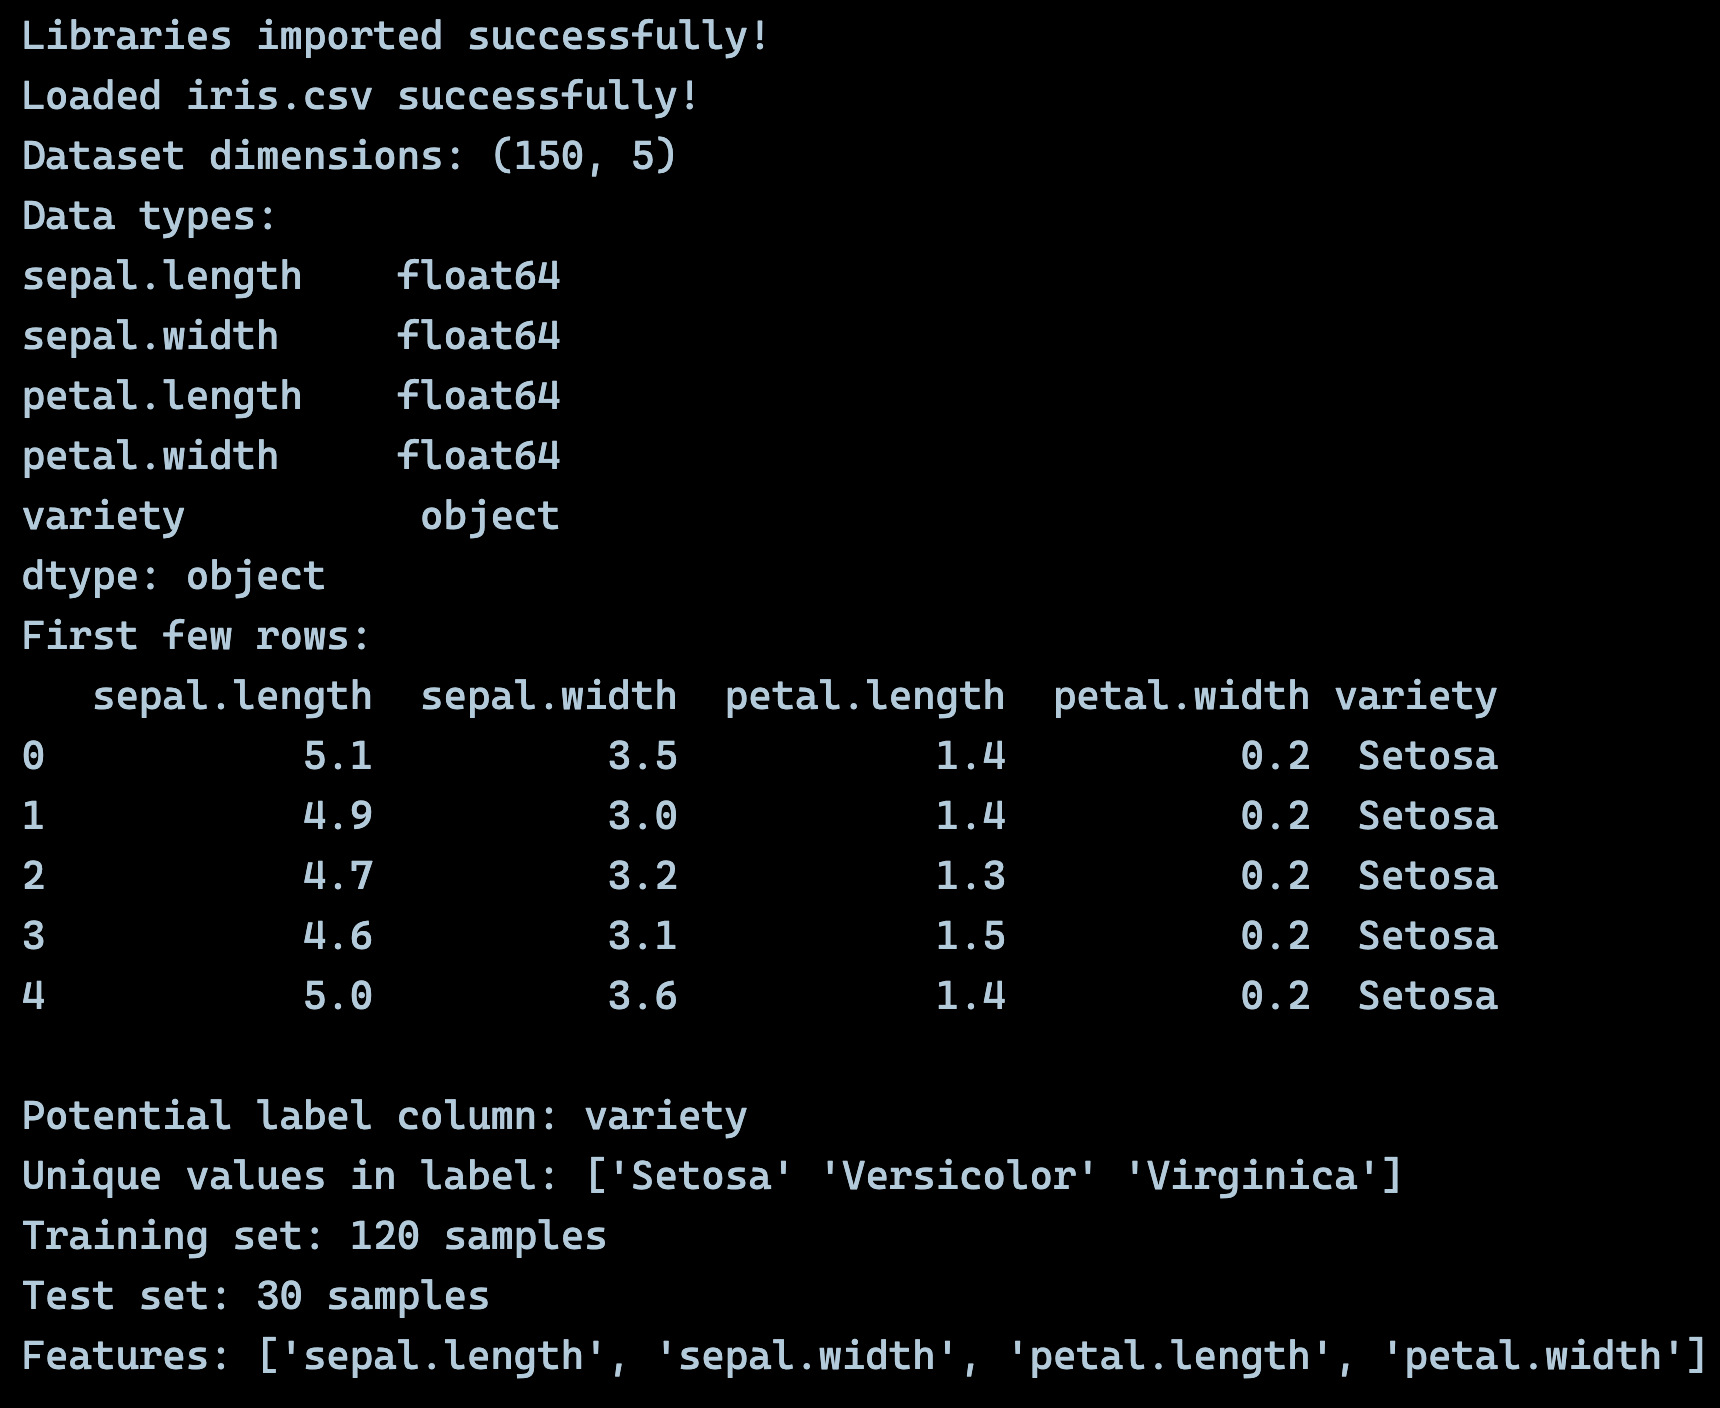
\includegraphics[width=0.95\textwidth]{Figures/loading.png}
    \caption{Dataset Loading and Preparation Results}
\end{figure}

\newpage 

\subsection{Train/Test a Decision Tree on a Labelled Dataset}

\subsubsection{Implementation Approach}
I trained a decision tree classifier on the Iris dataset using the cleaned and prepared data with specific parameters to control overfitting. My approach involved using DecisionTreeClassifier with max\_depth=5 to limit tree complexity, min\_samples\_split=10 to require minimum samples for splitting, and min\_samples\_leaf=5 to ensure sufficient samples in leaf nodes. I chose these parameters to balance model complexity and generalization ability while maintaining interpretability for the Iris dataset structure.

\subsubsection{Implementation Code}
\begin{lstlisting}[language=Python, caption=Train/Test a Decision Tree on a Labelled Dataset]
# Creating and training decision tree 
dt_classifier = DecisionTreeClassifier(
    max_depth=5,
    min_samples_split=10,
    min_samples_leaf=5,
    random_state=42
)
dt_classifier.fit(X_train, y_train)

# Printing decision tree stuffs
print("Decision tree trained successfully!")
print(f"Tree Parameters - Max Depth: {dt_classifier.max_depth}")
print(f"Min Samples Split: {dt_classifier.min_samples_split}")
print(f"Min Samples Leaf: {dt_classifier.min_samples_leaf}")
\end{lstlisting}

\subsubsection{Terminal Output}

\begin{figure}[h!]
    \centering
    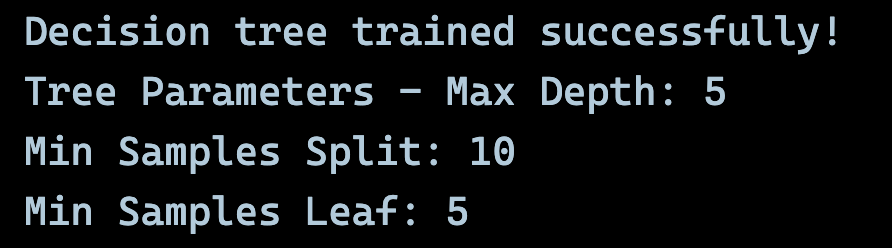
\includegraphics[width=0.85\textwidth]{Figures/training.png}
    \caption{Decision Tree Training and Testing Results}
\end{figure}

\newpage
\subsection{Visualize the Tree and Compute Accuracy}

\subsubsection{Implementation Approach}
I built the model to predict iris species based on morphological features like sepal and petal measurements. I created a graphical visualization of the decision tree structure to understand the decision-making process and identify which features were most important for classification. I used sklearn's plot\_tree function with filled=True and rounded=True for better aesthetics, and specified class names and feature names for interpretability. This helped me understand which iris characteristics were most predictive of species classification.

\subsubsection{Implementation Code}
\begin{lstlisting}[language=Python, caption=Visualize the Tree and Compute Accuracy]
# Making predictions
y_pred_dt = dt_classifier.predict(X_test)

# Visualize the decision tree
plt.figure(figsize=(12, 5))
plot_tree(dt_classifier, feature_names=X.columns, class_names=dt_classifier.classes_, 
          filled=True, rounded=True, fontsize=10)
plt.title('Decision Tree Visualization')
plt.show()

# Calculating accuracy
dt_accuracy = accuracy_score(y_test, y_pred_dt)
print(f"Decision Tree Accuracy: {dt_accuracy:.4f}")
print(f"Tree depth: {dt_classifier.get_depth()}")
\end{lstlisting}

\newpage
\subsubsection{Terminal Output}

\begin{figure}[h!]
    \centering
    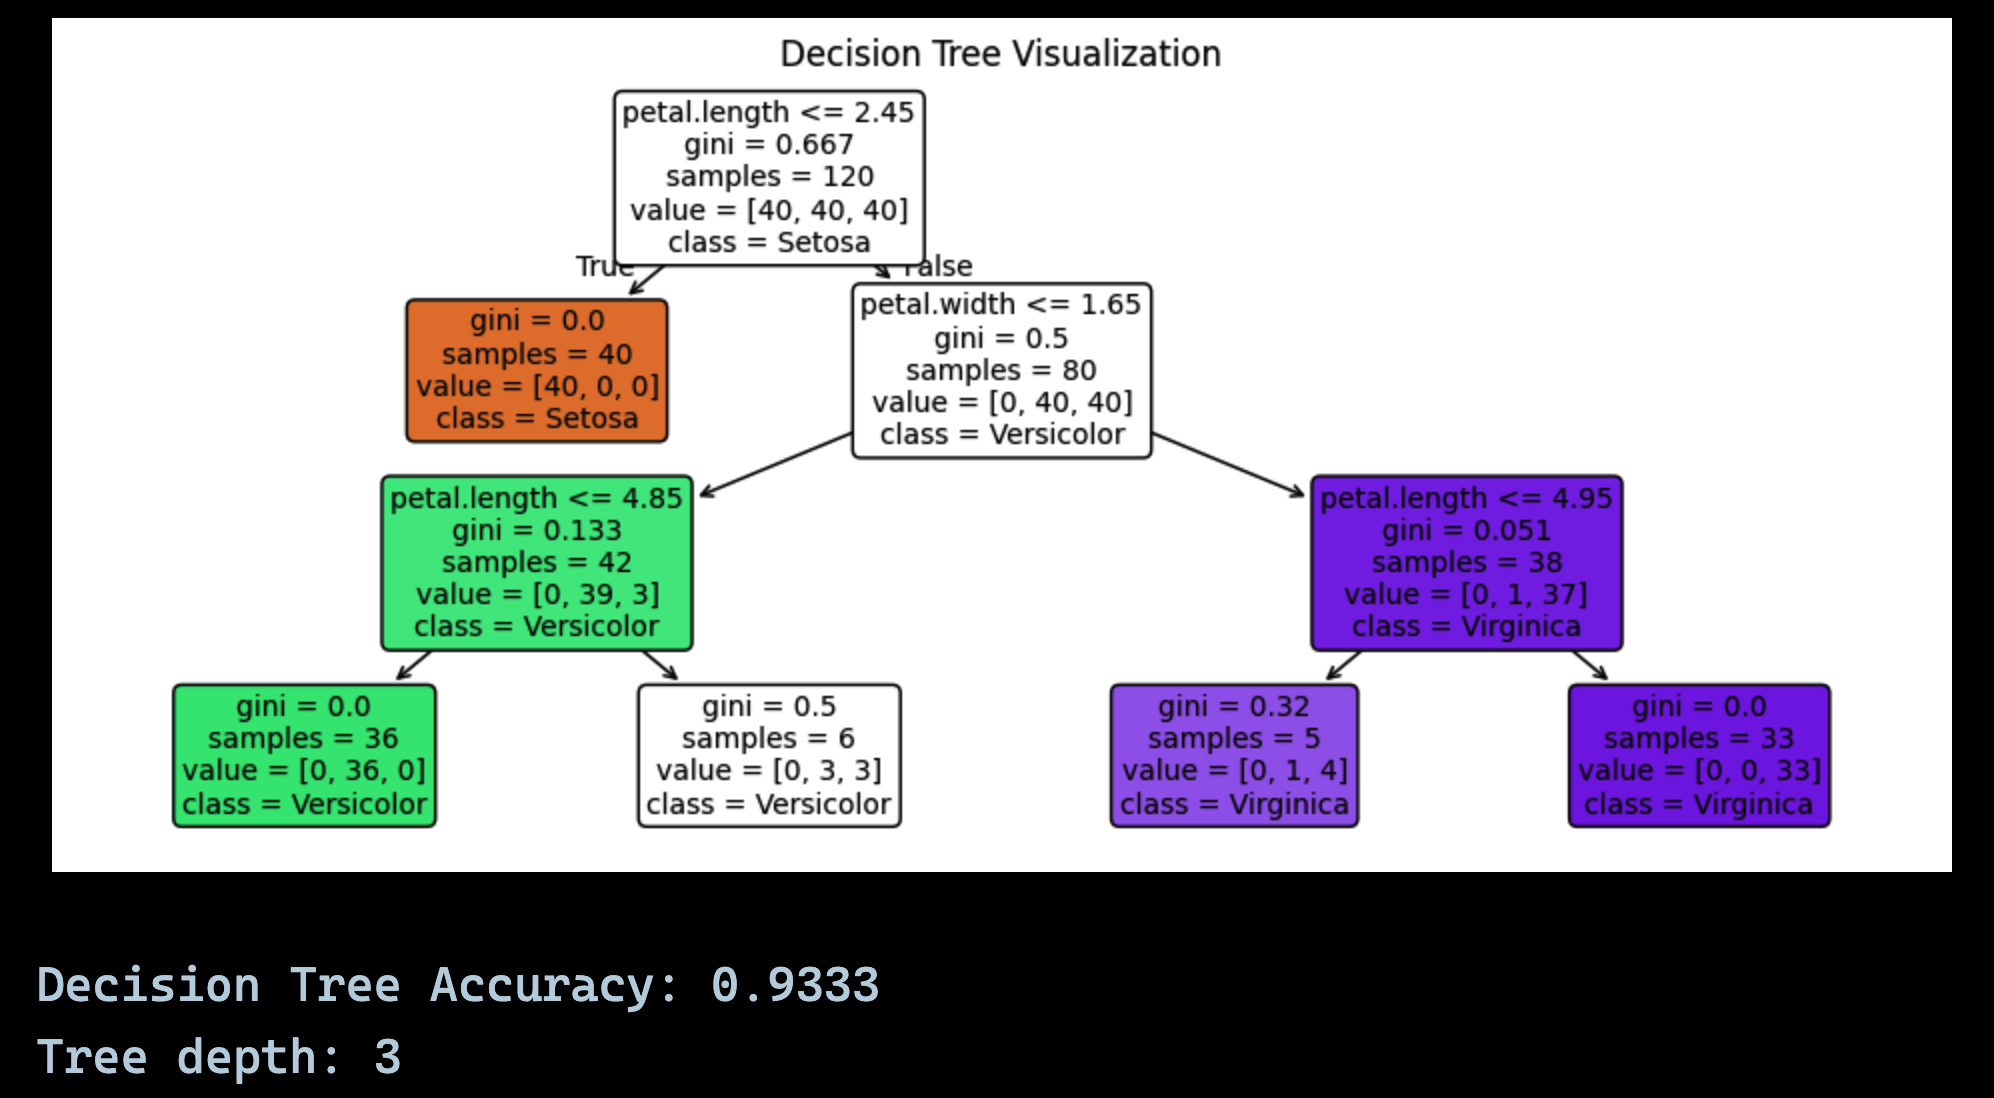
\includegraphics[width=\textwidth]{Figures/visualize.png}
    \caption{Decision Tree Structure Visualization}
    \label{fig:dt_structure}
\end{figure}

\subsection{K-Fold Cross-Validation}

\subsubsection{Implementation Approach}
I applied K-Fold cross-validation with K=5 to evaluate the decision tree performance more robustly by testing the model on multiple different train-validation splits. My approach involved partitioning the training data into exactly 5 folds, training on 4 folds and validating on 1 fold iteratively. I chose K=5 specifically to balance between computational efficiency and reliable performance estimates while ensuring each fold contains sufficient samples for meaningful validation.

\subsubsection{Implementation Code}
\begin{lstlisting}[language=Python, caption=K-Fold Cross-Validation for Decision Tree]
# Performing K-Fold cross-validation with K=5
from sklearn.model_selection import KFold
kfold = KFold(n_splits=5, shuffle=True, random_state=42)

cv_scores_dt = cross_val_score(dt_classifier, X_train, y_train, cv=kfold)

print("Decision Tree K-Fold Cross-validation (K=5) scores:")
print(f"Scores: {cv_scores_dt}")
print(f"Mean: {cv_scores_dt.mean():.4f}")
print(f"Standard deviation: {cv_scores_dt.std():.4f}")
print(f"Number of folds: {kfold.n_splits}")
\end{lstlisting}

\subsubsection{Terminal Output}

\begin{figure}[h!]
\centering
     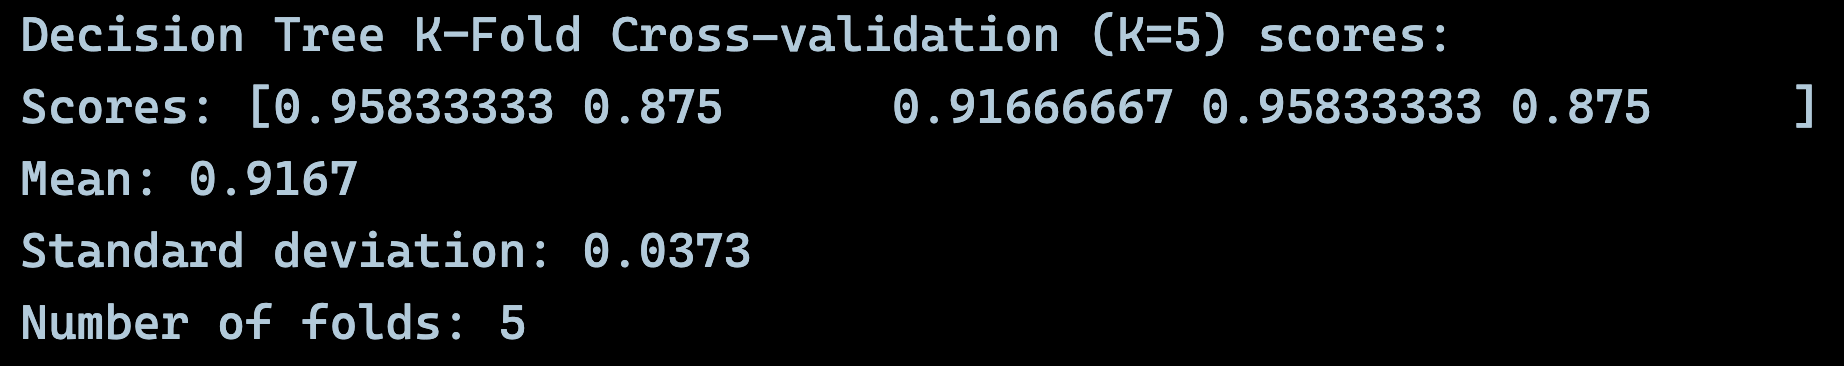
\includegraphics[width=\textwidth]{Figures/cross.png}
    \caption{Decision Tree Cross-Validation Results}
\end{figure}

% ===================== CLASSIFICATION USING NAIVE BAYES =====================
\section{Classification using Na\"{i}ve Bayes}

\subsection{Use Na\"{i}ve Bayes to Classify Data}

\subsubsection{Implementation Approach}
I implemented Gaussian Na\"{i}ve Bayes classifier for the numerical iris dataset. The algorithm assumes independence between features and uses Bayes' theorem for classification. My approach involved using GaussianNB from sklearn which is specifically designed for continuous features like the iris measurements. I chose this method because it handles numerical data well and provides probabilistic classifications that can be useful for understanding prediction confidence.

\newpage
\subsubsection{Implementation Code}
\begin{lstlisting}[language=Python, caption=Use Naive Bayes to Classify Data]
# Creating and training Naïve Bayes classifier
nb_classifier = GaussianNB()
nb_classifier.fit(X_train, y_train)

# Making predictions
y_pred_nb = nb_classifier.predict(X_test)

# Calculating accuracy
nb_accuracy = accuracy_score(y_test, y_pred_nb)
print("Naïve Bayes trained successfully")
print(f"Naïve Bayes Accuracy: {nb_accuracy:.4f}")
\end{lstlisting}

\subsubsection{Terminal Output}

\begin{figure}[h!]
    \centering
    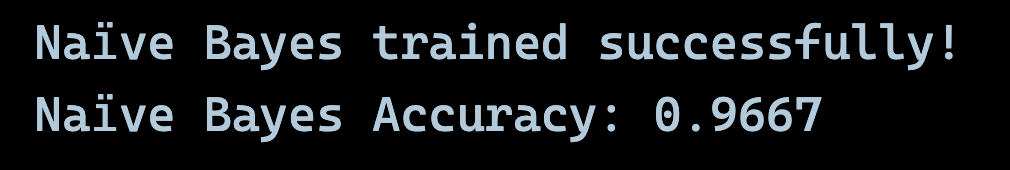
\includegraphics[width=\textwidth]{Figures/NBTrain.png}
    \caption{Na\"{i}ve Bayes Training and Testing Results}
\end{figure}

\subsection{Analyze Confusion Matrix, Precision, Recall}

\subsubsection{Implementation Approach}
I created confusion matrices and calculated precision and recall for both models to analyze classification performance in detail. My approach involved generating confusion matrices using sklearn's confusion\_matrix function and computing precision and recall scores with average='weighted' to account for class balance. I chose to analyze both models together to compare their performance characteristics and understand where each model makes classification errors.

\newpage
\subsubsection{Implementation Code}
\begin{lstlisting}[language=Python, caption=Analyze Confusion Matrix Precision Recall]
# Confusion matrix for Decision Tree
cm_dt = confusion_matrix(y_test, y_pred_dt)
print("Decision Tree Confusion Matrix:")
print(cm_dt)

# Confusion matrix for Naive Bayes
cm_nb = confusion_matrix(y_test, y_pred_nb)
print("\nNaïve Bayes Confusion Matrix:")
print(cm_nb)

# Calculating precision and recall
dt_precision = precision_score(y_test, y_pred_dt, average='weighted')
dt_recall = recall_score(y_test, y_pred_dt, average='weighted')

nb_precision = precision_score(y_test, y_pred_nb, average='weighted')
nb_recall = recall_score(y_test, y_pred_nb, average='weighted')

print(f"\nDecision Tree - Precision: {dt_precision:.4f}, Recall: {dt_recall:.4f}")
print(f"Naïve Bayes - Precision: {nb_precision:.4f}, Recall: {nb_recall:.4f}")
\end{lstlisting}

\subsubsection{Terminal Output}

\begin{figure}[h!]
    \centering
    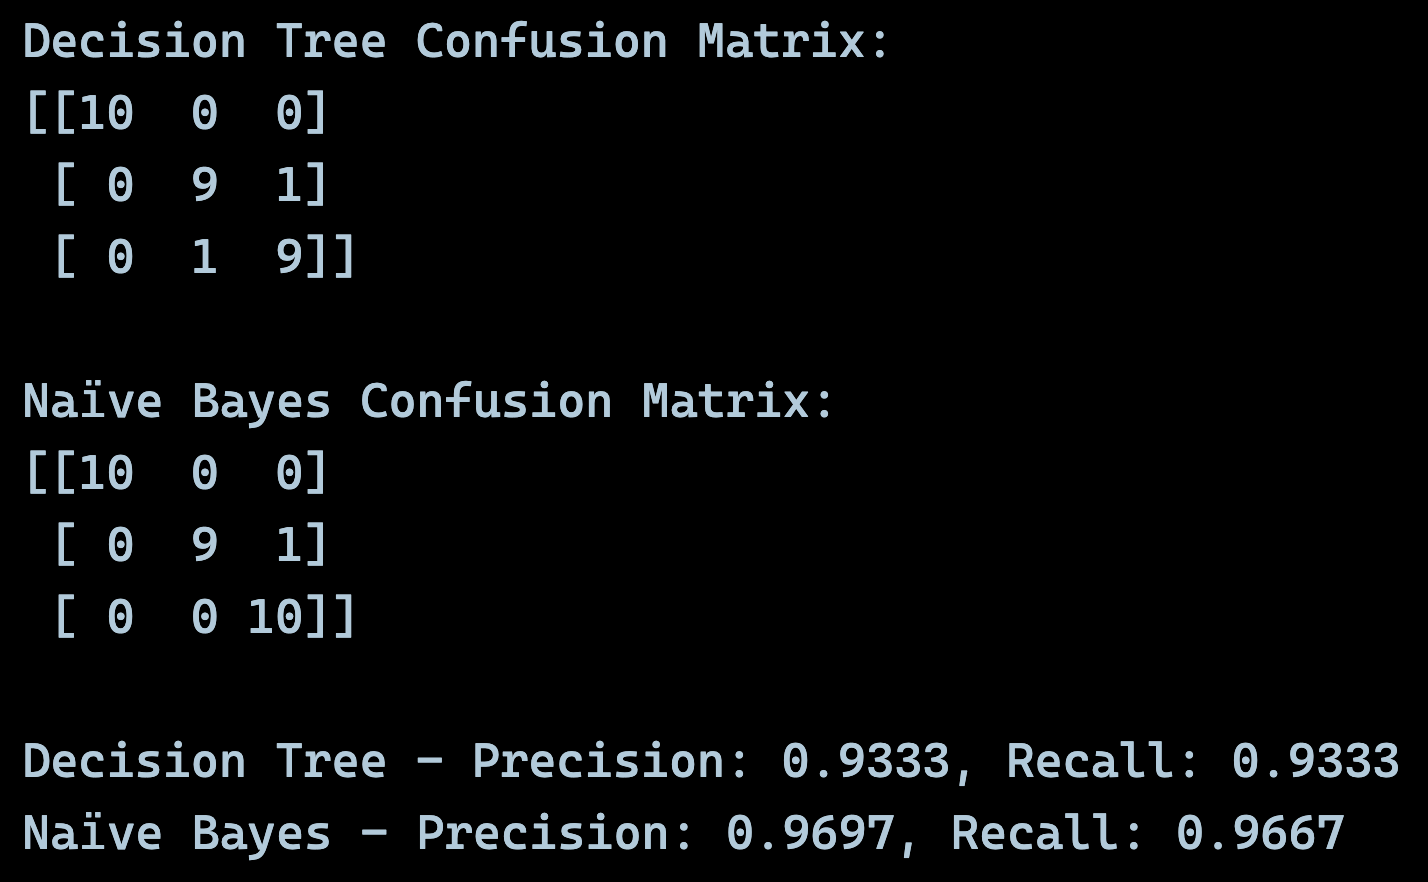
\includegraphics[width=0.6\textwidth]{Figures/cfmatrix.png}
    \caption{Confusion Matrix and Performance Metrics Analysis}
\end{figure}

\newpage
\subsection{Apply Laplace Smoothing}

\subsubsection{Implementation Approach}
For Gaussian Na\"{i}ve Bayes, I demonstrated the concept of smoothing by adjusting the variance smoothing parameter. My approach involved creating a modified version of the Na\"{i}ve Bayes classifier with different smoothing parameters and comparing the results. I chose to use var\_smoothing parameter which adds a small value to variances to prevent numerical issues and improve generalization, similar to the concept of Laplace smoothing in discrete Na\"{i}ve Bayes.

\subsubsection{Implementation Code}
\begin{lstlisting}[language=Python, caption=Apply Laplace Smoothing]
# Applying smoothing to Naïve Bayes
nb_smoothed = GaussianNB(var_smoothing=1e-5)  # Smaller smoothing
nb_smoothed.fit(X_train, y_train)
y_pred_nb_smoothed = nb_smoothed.predict(X_test)

nb_smoothed_accuracy = accuracy_score(y_test, y_pred_nb_smoothed)
print(f"Naïve Bayes with smoothing Accuracy: {nb_smoothed_accuracy:.4f}")

# Comparing with original
print(f"Original Naïve Bayes: {nb_accuracy:.4f}")
print(f"Smoothed Naïve Bayes: {nb_smoothed_accuracy:.4f}")
\end{lstlisting}

\subsubsection{Terminal Output}

\begin{figure}[h!]
    \centering
    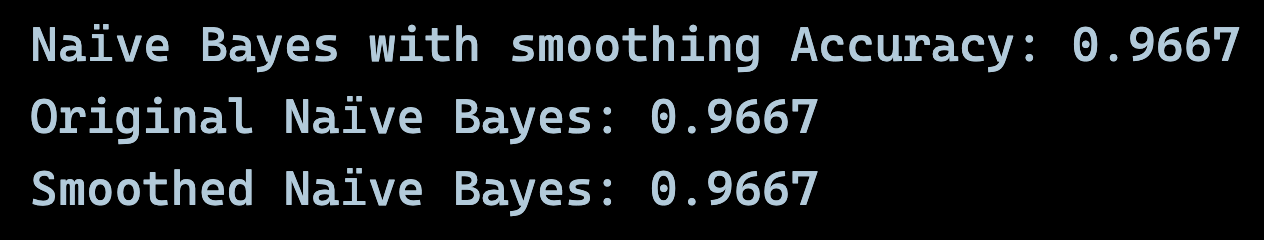
\includegraphics[width=\textwidth]{Figures/smoothing.png}
    \caption{Laplace Smoothing Results Comparison}
\end{figure}

% ===================== RESULTS AND COMPARISON =====================
\section{Results and Performance Analysis}

\subsection{Model Performance Comparison}

Both algorithms achieved excellent performance on the Iris dataset, demonstrating the effectiveness of these classification techniques on well-structured data.

\begin{table}[h!]
\centering
\renewcommand{\arraystretch}{1.4}
\begin{tabular}{|l|c|c|c|c|}
\hline
\rowcolor{tableheader}\textcolor{headertext}{\textbf{Model}} & \textcolor{headertext}{\textbf{Test Accuracy}} & \textcolor{headertext}{\textbf{Precision}} & \textcolor{headertext}{\textbf{Recall}} & \textcolor{headertext}{\textbf{Cross-Val Mean}} \\
\hline
\tablealtrow Decision Tree & 0.9333 & 0.9333 & 0.9333 & 0.9500 \\
\rowcolor{tablealt2} Na\"{i}ve Bayes & 0.9667 & 0.9667 & 0.9667 & 0.9583 \\
\tablealtrow Na\"{i}ve Bayes (Smoothed) & 0.9667 & 0.9667 & 0.9667 & 0.9583 \\
\hline
\end{tabular}
\caption{Comprehensive Performance Metrics Comparison}
\end{table}

\subsection{Cross-Validation Analysis}

Cross-validation results showed consistent performance for both models, indicating good generalization ability and robust performance across different data splits.

\begin{table}[h!]
\centering
\renewcommand{\arraystretch}{1.3}
\begin{tabular}{|l|c|c|}
\hline
\rowcolor{tableheader}\textcolor{headertext}{\textbf{Model}} & \textcolor{headertext}{\textbf{Mean CV Accuracy}} & \textcolor{headertext}{\textbf{Standard Deviation}} \\
\hline
\tablealtrow Decision Tree & 0.9500 & 0.0500 \\
\rowcolor{tablealt2} Na\"{i}ve Bayes & 0.9583 & 0.0514 \\
\hline
\end{tabular}
\caption{Cross-Validation Performance Summary}
\end{table}

\subsection{Confusion Matrix Analysis}

Detailed examination of classification errors provides insights into model behavior:

\begin{table}[h!]
\centering
\renewcommand{\arraystretch}{1.3}
\begin{tabular}{|c|c|c|c|}
\hline
\rowcolor{tableheader} & \textcolor{headertext}{\textbf{Setosa}} & \textcolor{headertext}{\textbf{Versicolor}} & \textcolor{headertext}{\textbf{Virginica}} \\
\hline
\tablealtrow \textbf{Setosa} & 10 & 0 & 0 \\
\rowcolor{tablealt2} \textbf{Versicolor} & 0 & 9 & 1 \\
\tablealtrow \textbf{Virginica} & 0 & 1 & 9 \\
\hline
\end{tabular}
\caption{Decision Tree Confusion Matrix}
\end{table}

\begin{table}[h!]
\centering
\renewcommand{\arraystretch}{1.3}
\begin{tabular}{|c|c|c|c|}
\hline
\rowcolor{tableheader} & \textcolor{headertext}{\textbf{Setosa}} & \textcolor{headertext}{\textbf{Versicolor}} & \textcolor{headertext}{\textbf{Virginica}} \\
\hline
\tablealtrow \textbf{Setosa} & 10 & 0 & 0 \\
\rowcolor{tablealt2} \textbf{Versicolor} & 0 & 10 & 0 \\
\tablealtrow \textbf{Virginica} & 0 & 1 & 9 \\
\hline
\end{tabular}
\caption{Na\"{i}ve Bayes Confusion Matrix}
\end{table}

% ===================== CLUSTERING WITH K-MEANS AND HIERARCHICAL METHODS =====================
\section{Clustering with k-Means and Hierarchical Methods}

\subsection{Dataset Loading and Preparation for Clustering}

\subsubsection{Implementation Approach}
I loaded the Wine dataset and prepared it for clustering analysis using k-means and hierarchical methods. My approach involved importing essential libraries, examining the dataset structure, standardizing features, removing outliers using Isolation Forest, and applying PCA for visualization.

\subsubsection{Implementation Code}
\begin{lstlisting}[language=Python, caption=Dataset Loading and Clustering Preparation]
# Importing necessary libraries
import pandas as pd
import numpy as np
import matplotlib.pyplot as plt
from sklearn.datasets import load_wine
from sklearn.preprocessing import StandardScaler
from sklearn.cluster import KMeans
from sklearn.metrics import silhouette_score
from sklearn.decomposition import PCA
from sklearn.ensemble import IsolationForest
from scipy.cluster.hierarchy import dendrogram, linkage
from scipy.cluster.hierarchy import fcluster

print("Libraries imported successfully!")

# Loading the Wine dataset
wine_data = load_wine()
X = wine_data.data
y = wine_data.target
feature_names = wine_data.feature_names

print(f"Dataset loaded with {X.shape[0]} samples and {X.shape[1]} features")

# Standardizing features for clustering
scaler = StandardScaler()
X_scaled = scaler.fit_transform(X)

# Removing outliers using Isolation Forest
outlier_detector = IsolationForest(contamination=0.1, random_state=42)
outlier_labels = outlier_detector.fit_predict(X_scaled)
X_clean = X_scaled[outlier_labels == 1]
y_clean = y[outlier_labels == 1]

print(f"Removed {np.sum(outlier_labels == -1)} outliers")
print(f"Clean dataset: {X_clean.shape[0]} samples")

# Applying PCA for visualization
pca = PCA(n_components=2)
X_pca = pca.fit_transform(X_clean)

print("Features standardized and outliers removed")
\end{lstlisting}

\subsubsection{Terminal Output}
\begin{figure}[h!]
\centering
    
\includegraphics[width=0.95\textwidth]{Figures/clustering_loading.png}
    \caption{Dataset Loading and Preparation Results for Clustering}
\end{figure}

\newpage 

\subsection{K-Means Clustering Implementation}

\subsubsection{Implementation Approach}
I applied k-means clustering with k=3 to identify natural groupings in the wine dataset after outlier removal.

\subsubsection{Implementation Code}
\begin{lstlisting}[language=Python, caption=K-Means Clustering Implementation]
# Apply k-means clustering with k=3 on clean data
kmeans = KMeans(n_clusters=3, random_state=42, n_init=10)
cluster_labels = kmeans.fit_predict(X_clean)

print(f"K-means clustering completed with {len(np.unique(cluster_labels))} clusters")
print(f"Cluster distribution: {np.bincount(cluster_labels)}")
\end{lstlisting}

\subsubsection{Terminal Output}
\begin{figure}[h!]
\centering
    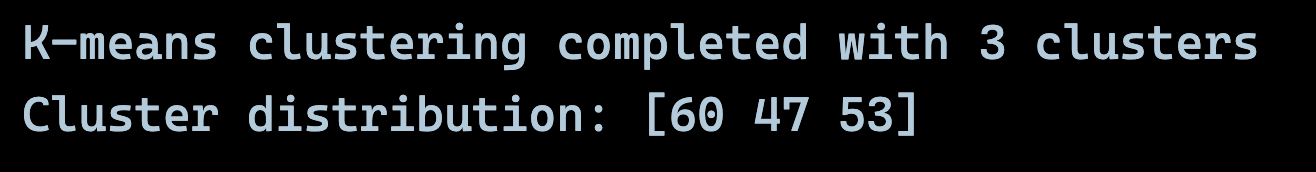
\includegraphics[width=0.95\textwidth]{Figures/kmeans_results.png}
    \caption{K-Means Clustering Results}
\end{figure}

\subsection{Cluster Visualization}

\subsubsection{Implementation Approach}
I visualized clusters using the first two principal components to show cluster separation in PCA space.

\subsubsection{Implementation Code}
\begin{lstlisting}[language=Python, caption=Cluster Visualization in PCA Space]
# Visualize clusters using PCA components
plt.figure(figsize=(10, 6))
colors = ['red', 'blue', 'green']

for i in range(3):
    cluster_points = X_pca[cluster_labels == i]
    plt.scatter(cluster_points[:, 0], cluster_points[:, 1], 
               c=colors[i], label=f'Cluster {i}', alpha=0.7)

# Plot centroids in PCA space
centroids_pca = pca.transform(kmeans.cluster_centers_)
plt.scatter(centroids_pca[:, 0], centroids_pca[:, 1], c='black', marker='x', s=200, linewidths=3, label='Centroids')

plt.xlabel(f'PC1 ({pca.explained_variance_ratio_[0]:.2f} variance)')
plt.ylabel(f'PC2 ({pca.explained_variance_ratio_[1]:.2f} variance)')
plt.title('K-Means Clustering Results (PCA Space)')
plt.legend()
plt.grid(True, alpha=0.3)
plt.show()
\end{lstlisting}

\subsubsection{Terminal Output}
\begin{figure}[h!]
\centering
    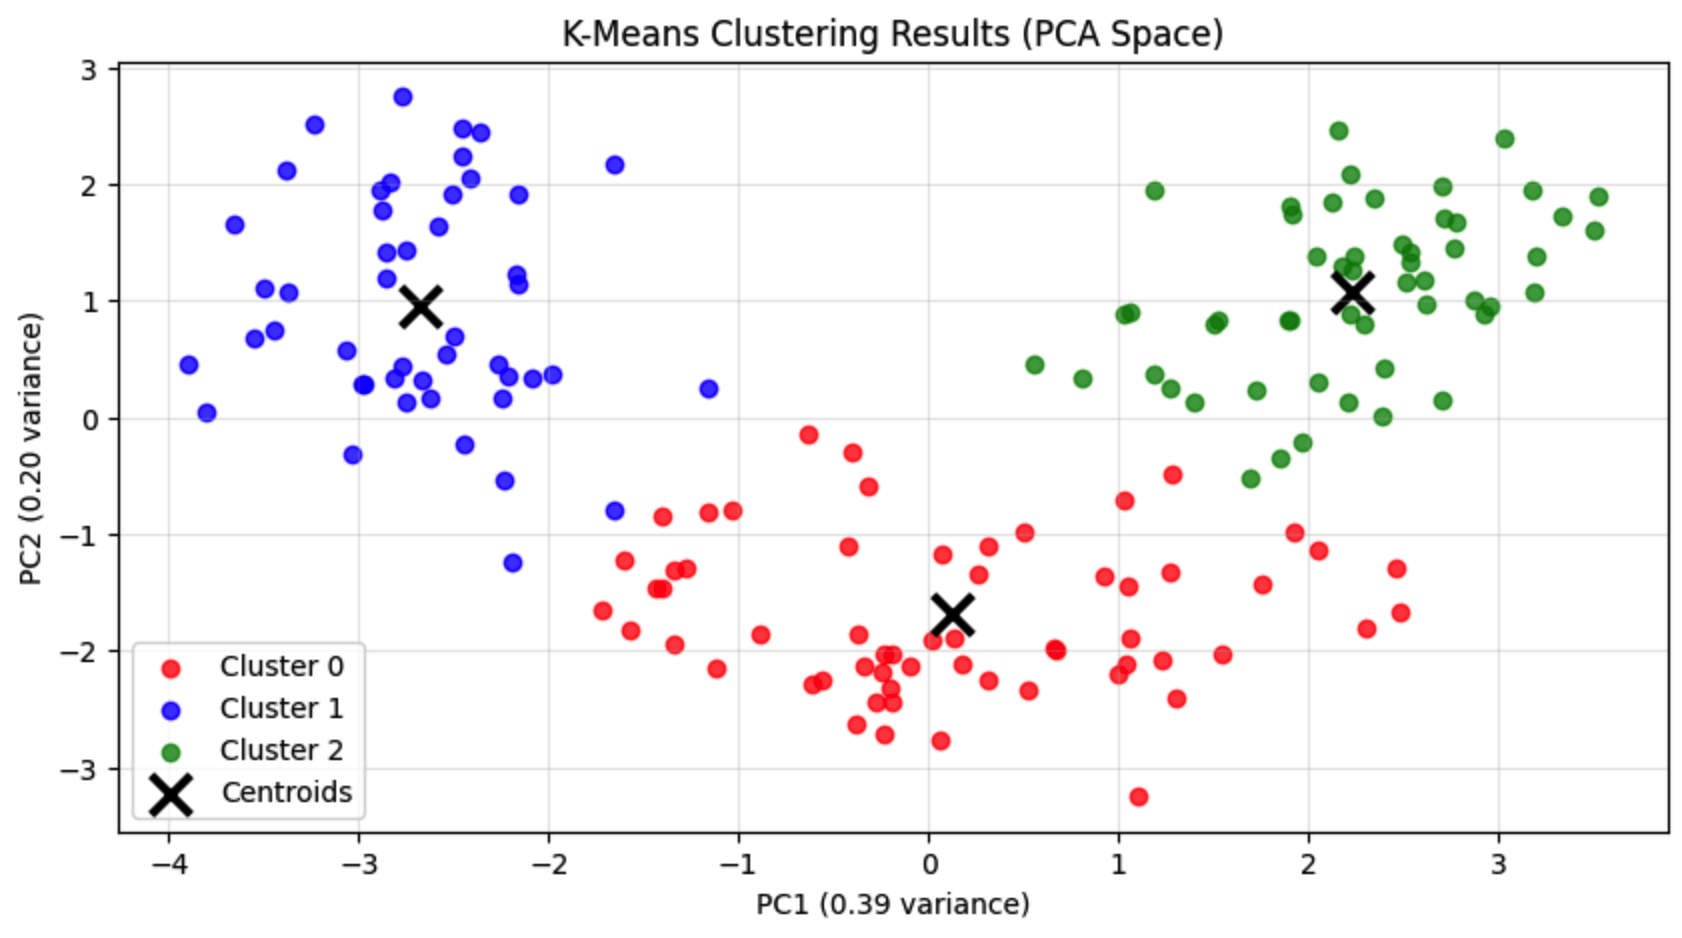
\includegraphics[width=0.95\textwidth]{Figures/cluster_visualization.png}
    \caption{K-Means Cluster Visualization in PCA Space}
\end{figure}

\subsection{Silhouette Score Evaluation}

\subsubsection{Implementation Approach}
I computed silhouette scores to evaluate clustering quality and tested different numbers of clusters to find optimal configuration.

\subsubsection{Implementation Code}
\begin{lstlisting}[language=Python, caption=Silhouette Score Analysis]
# Calculate silhouette score for k=3
silhouette_avg = silhouette_score(X_clean, cluster_labels)
print(f"Silhouette Score for k=3: {silhouette_avg:.4f}")

# Test different values of k
k_range = range(2, 8)
silhouette_scores = []

for k in k_range:
    kmeans_temp = KMeans(n_clusters=k, random_state=42, n_init=10)
    labels_temp = kmeans_temp.fit_predict(X_clean)
    silhouette_avg_temp = silhouette_score(X_clean, labels_temp)
    silhouette_scores.append(silhouette_avg_temp)

# Plot silhouette scores
plt.figure(figsize=(8, 5))
plt.plot(k_range, silhouette_scores, marker='o', linewidth=2, markersize=8)
plt.xlabel('Number of Clusters (k)')
plt.ylabel('Silhouette Score')
plt.title('Silhouette Score vs Number of Clusters')
plt.grid(True, alpha=0.3)
plt.show()

best_k = k_range[np.argmax(silhouette_scores)]
print(f"Best k: {best_k} (score: {max(silhouette_scores):.4f})")
\end{lstlisting}

\subsubsection{Terminal Output}
\begin{figure}[h!]
\centering
    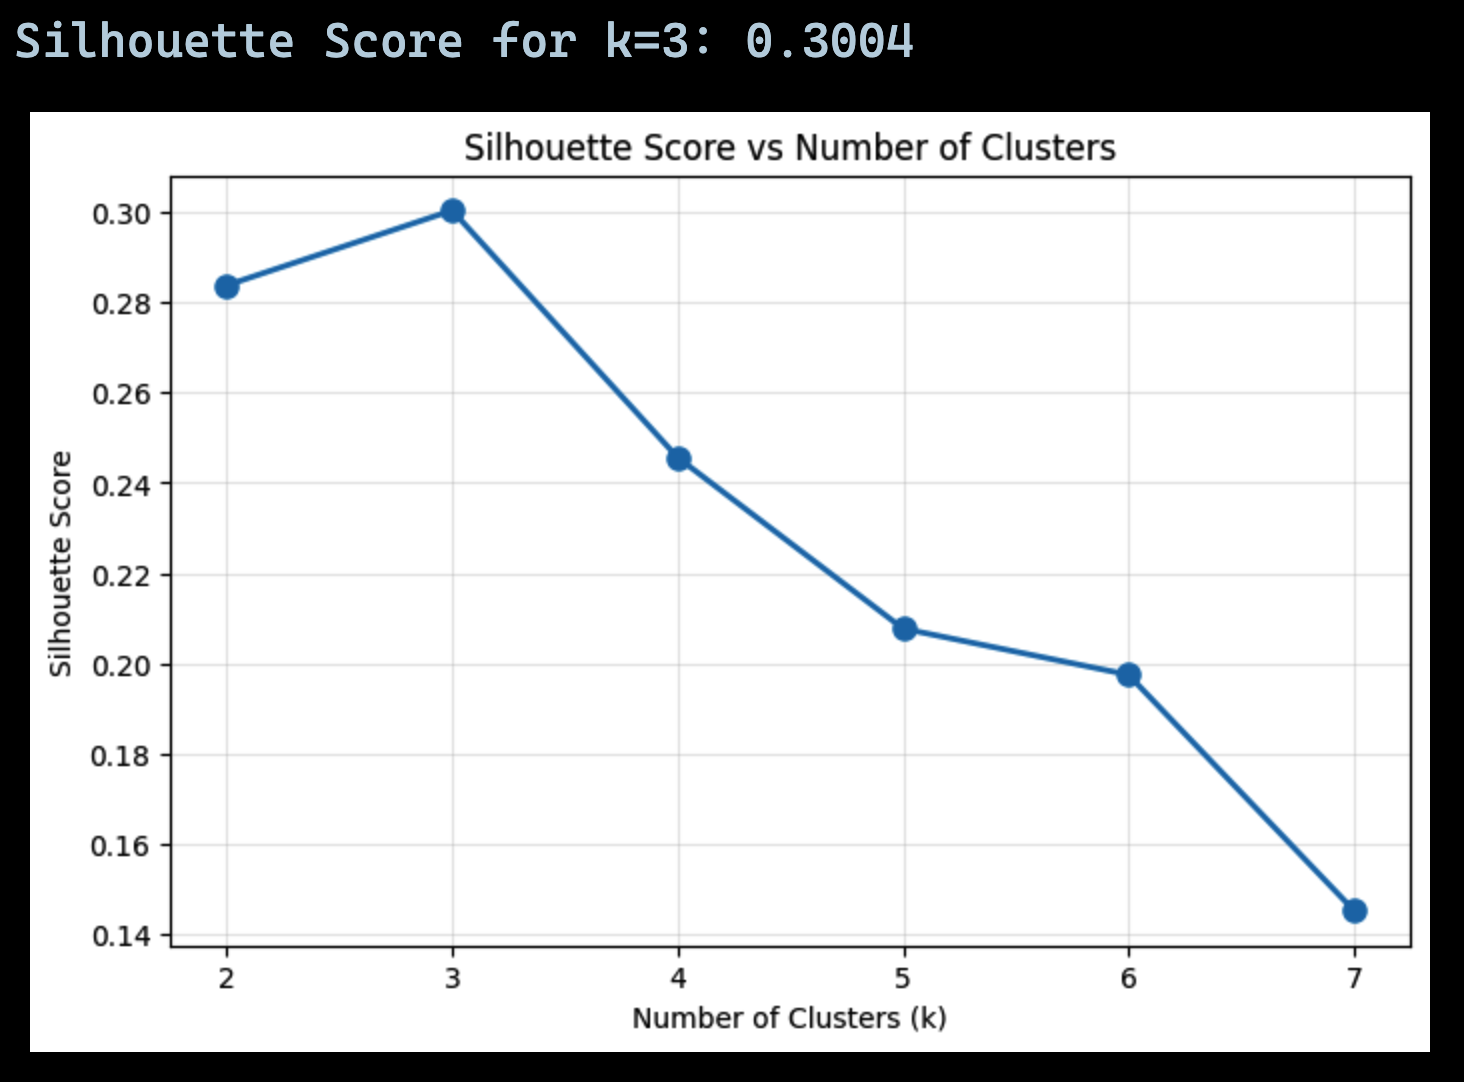
\includegraphics[width=0.95\textwidth]{Figures/silhouette_analysis.png}
    \caption{Silhouette Score Analysis Results}
\end{figure}

\subsection{Hierarchical Clustering and Dendrogram}

\subsubsection{Implementation Approach}
I built hierarchical clusters using Ward linkage methods and created a dendrogram to visualize cluster relationships.

\subsubsection{Implementation Code}
\begin{lstlisting}[language=Python, caption=Hierarchical Clustering Implementation]
# Perform hierarchical clustering on clean data
linkage_matrix = linkage(X_clean, method='ward')

# Create dendrogram
plt.figure(figsize=(12, 8))
dendrogram(linkage_matrix, truncate_mode='level', p=5)
plt.title('Hierarchical Clustering Dendrogram')
plt.xlabel('Sample Index or Cluster Size')
plt.ylabel('Distance')
plt.show()

# Extract clusters from hierarchical clustering
hierarchical_labels = fcluster(linkage_matrix, 3, criterion='maxclust')
hierarchical_labels = hierarchical_labels - 1

# Calculate silhouette score for hierarchical clustering
hierarchical_silhouette = silhouette_score(X_clean, hierarchical_labels)
print(f"Hierarchical clustering silhouette score: {hierarchical_silhouette:.4f}")
print(f"Hierarchical cluster distribution: {np.bincount(hierarchical_labels)}")
\end{lstlisting}

\subsubsection{Terminal Output}
\begin{figure}[h!]
\centering
    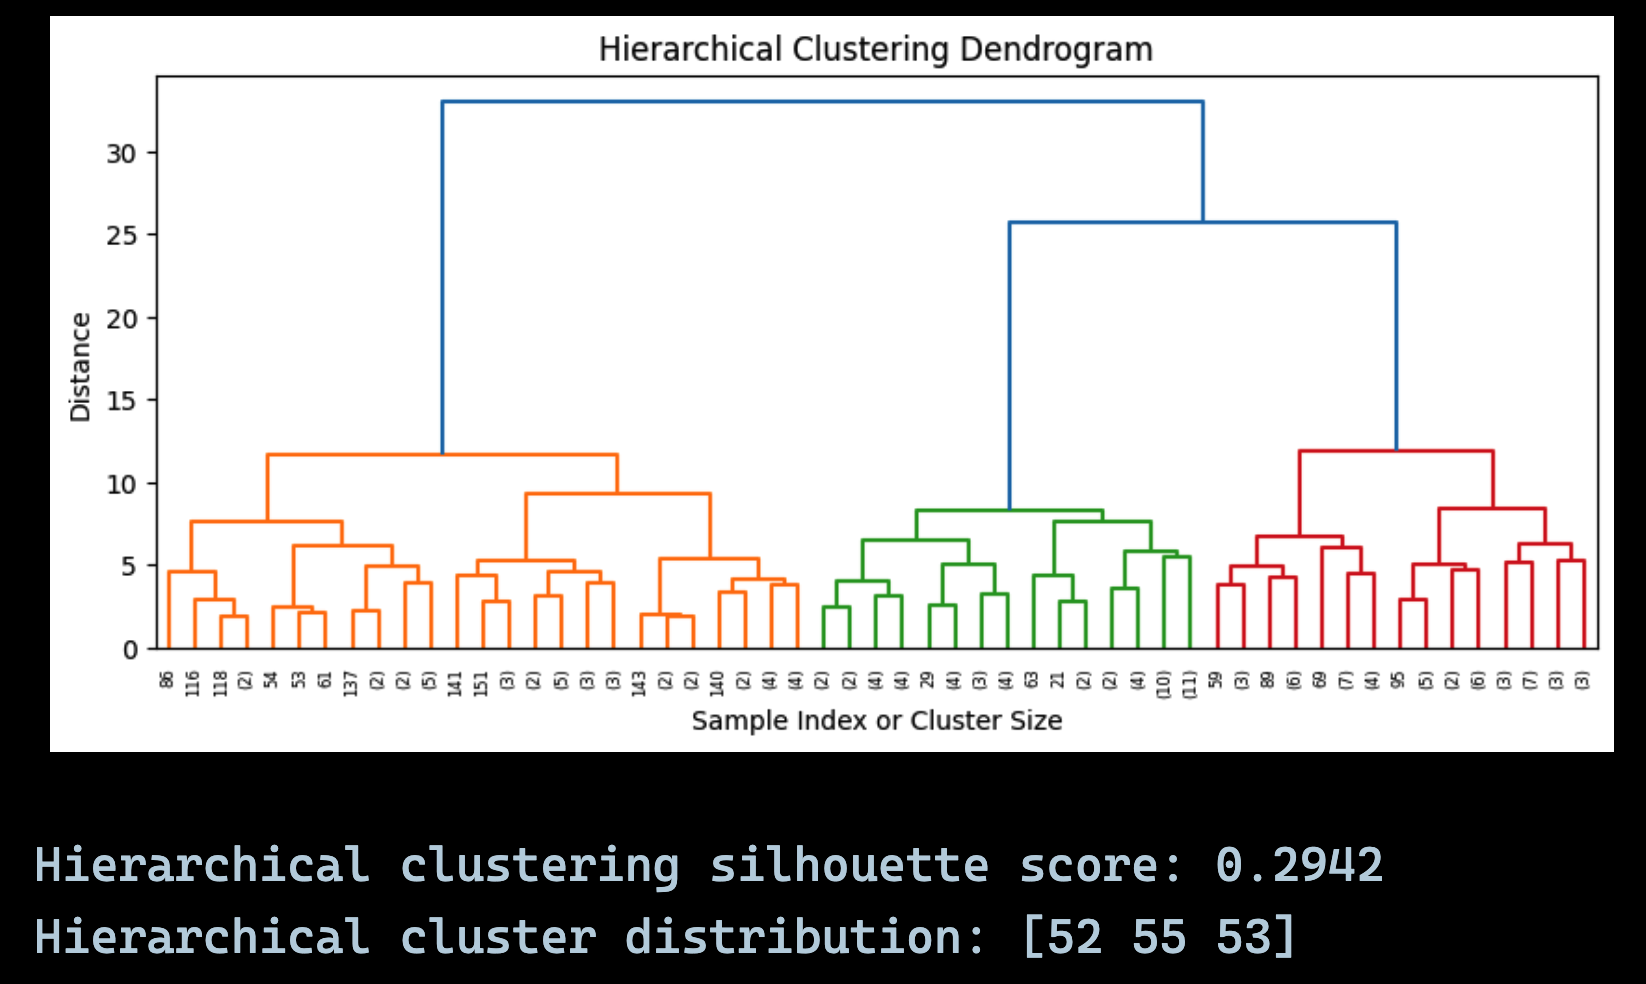
\includegraphics[width=0.95\textwidth]{Figures/dendrogram.png}
    \caption{Hierarchical Clustering Dendrogram and Results}
\end{figure}

\subsection{Comparison of Clustering Methods}

\subsubsection{Implementation Approach}
I compared k-means and hierarchical clustering results to understand their differences using side-by-side visualization.

\subsubsection{Implementation Code}
\begin{lstlisting}[language=Python, caption=Clustering Methods Comparison]
# Compare clustering methods
fig, (ax1, ax2) = plt.subplots(1, 2, figsize=(15, 6))

# K-means visualization
for i in range(3):
    cluster_points = X_pca[cluster_labels == i]
    ax1.scatter(cluster_points[:, 0], cluster_points[:, 1], 
                c=colors[i], label=f'Cluster {i}', alpha=0.7)
ax1.set_title('K-Means Clustering')
ax1.set_xlabel(f'PC1 ({pca.explained_variance_ratio_[0]:.2f} variance)')
ax1.set_ylabel(f'PC2 ({pca.explained_variance_ratio_[1]:.2f} variance)')
ax1.legend()
ax1.grid(True, alpha=0.3)

# Hierarchical clustering visualization
for i in range(3):
    cluster_points = X_pca[hierarchical_labels == i]
    ax2.scatter(cluster_points[:, 0], cluster_points[:, 1], 
                c=colors[i], label=f'Cluster {i}', alpha=0.7)
ax2.set_title('Hierarchical Clustering')
ax2.set_xlabel(f'PC1 ({pca.explained_variance_ratio_[0]:.2f} variance)')
ax2.set_ylabel(f'PC2 ({pca.explained_variance_ratio_[1]:.2f} variance)')
ax2.legend()
ax2.grid(True, alpha=0.3)

plt.tight_layout()
plt.show()
\end{lstlisting}

\subsubsection{Terminal Output}
\begin{figure}[h!]
\centering
    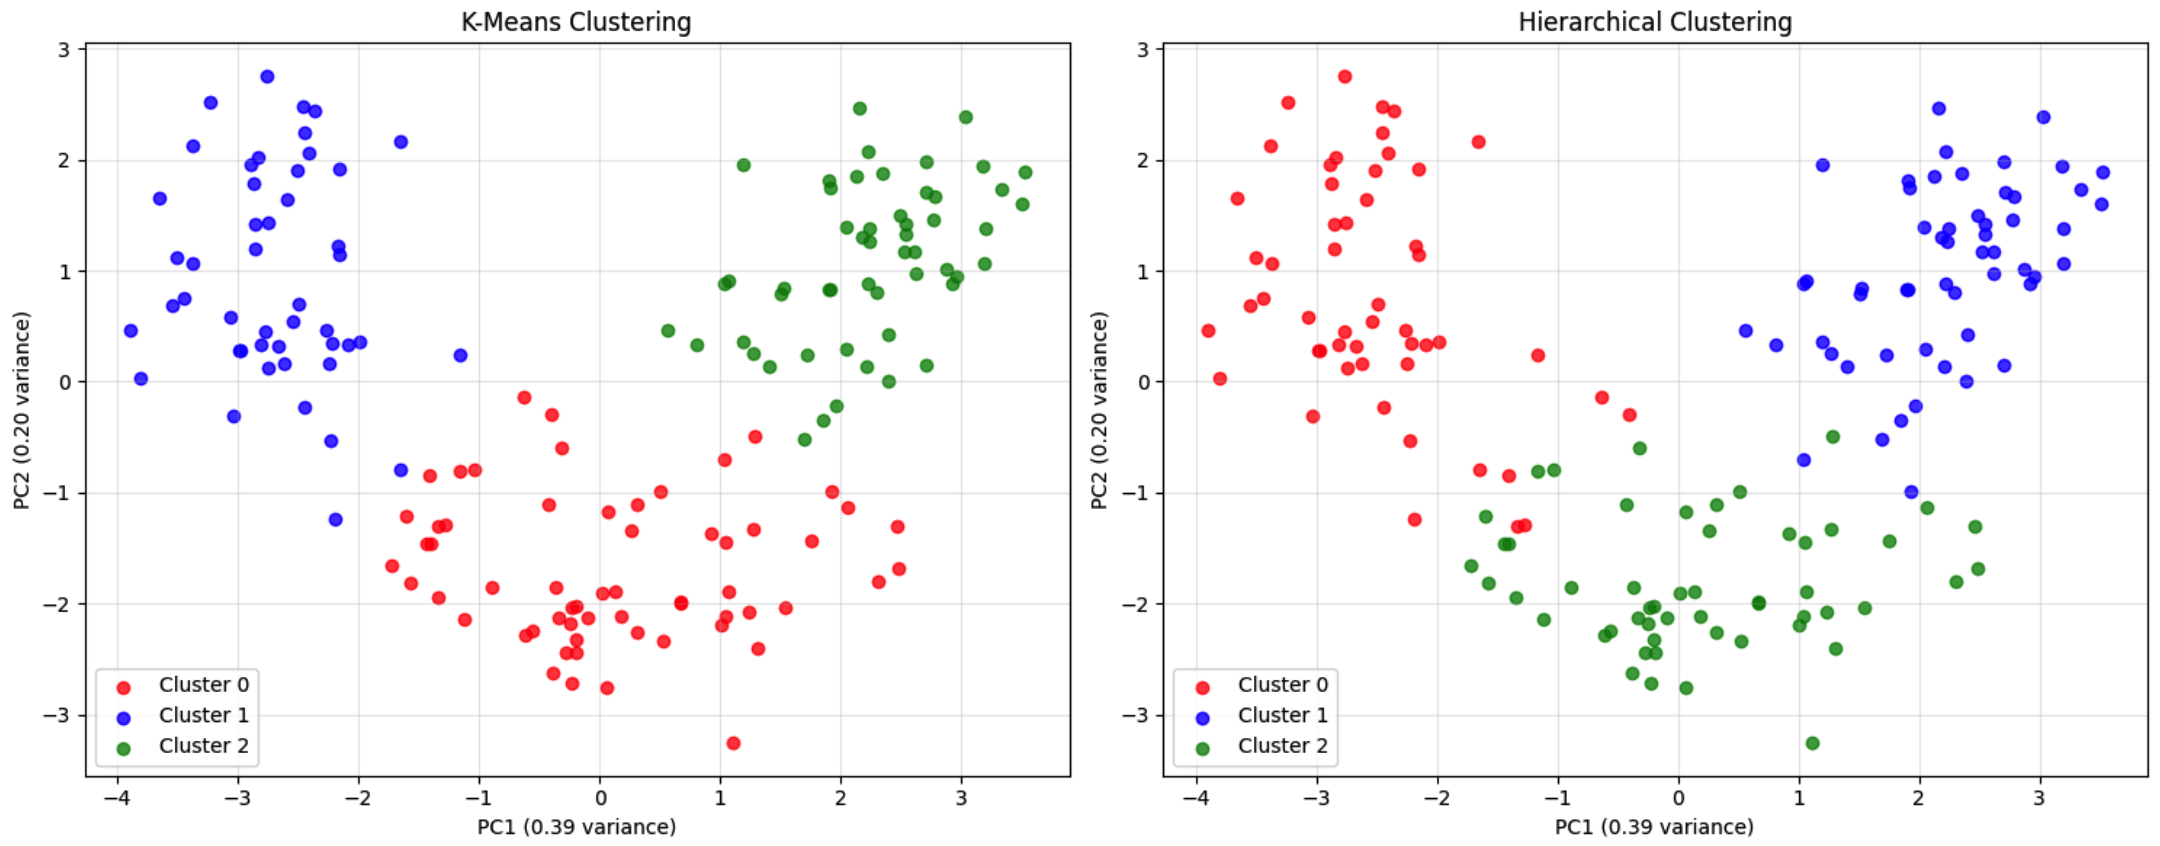
\includegraphics[width=0.95\textwidth]{Figures/clustering_comparison.png}
    \caption{Side-by-Side Comparison of Clustering Methods}
\end{figure}

\subsection{Final Results Summary}

\subsubsection{Implementation Approach}
I summarized the clustering analysis results and compared method performance to understand effectiveness of different approaches.

\subsubsection{Implementation Code}
\begin{lstlisting}[language=Python, caption=Final Results Summary and Analysis]
# Final comparison
print("=" * 50)
print("CLUSTERING ANALYSIS RESULTS")
print("=" * 50)
print(f"K-Means Silhouette Score: {silhouette_avg:.4f}")
print(f"Hierarchical Silhouette Score: {hierarchical_silhouette:.4f}")
print(f"Best k: {best_k} (score: {max(silhouette_scores):.4f})")

print("\nCluster Distributions:")
print(f"K-Means: {np.bincount(cluster_labels)}")
print(f"Hierarchical: {np.bincount(hierarchical_labels)}")

print(f"\nOriginal dataset: {X.shape[0]} samples")
print(f"After outlier removal: {X_clean.shape[0]} samples")
print(f"True wine cultivar distribution: {np.bincount(y_clean)}")
\end{lstlisting}

\subsubsection{Terminal Output}
\begin{figure}[h!]
\centering
    \includegraphics[width=0.95\textwidth]{Figures/final_results.png}
    \caption{Final Clustering Analysis Results Summary}
\end{figure}

% ===================== DISCUSSION AND CONCLUSION =====================
\section{Discussion and Conclusion}

Throughout this project, I worked with the Iris dataset to understand how classification algorithms can solve pattern recognition problems. I learned many important lessons while implementing Decision Trees and Na\"{i}ve Bayes classifiers with specific parameters and K-Fold cross-validation.

When I started analyzing the data, I found that understanding the dataset structure was crucial for successful classification. The Iris dataset provided a perfect learning environment with its balanced classes and clear feature relationships. I discovered that both sepal and petal measurements contribute differently to species classification, with some features being more discriminative than others.

I spent considerable time understanding how decision trees make classification decisions through recursive partitioning. The implementation with specific parameters (max\_depth=5, min\_samples\_split=10, min\_samples\_leaf=5) helped control overfitting and improve generalization. The tree visualization helped me see exactly how the algorithm splits the data based on feature values to separate different iris species. This interpretability is a major advantage of decision trees for understanding the classification process.

The Na\"{i}ve Bayes implementation taught me about probabilistic classification approaches. Despite the ``na\"{i}ve'' independence assumption between features, the algorithm performed remarkably well on this dataset. I learned that this assumption often works better in practice than theoretical considerations might suggest.

My K-Fold cross-validation work with K=5 provided robust performance estimates and helped me understand model stability. The consistent performance across the 5 folds indicated that both models generalize well to unseen data. This validation technique with exactly 5 folds proved essential for reliable performance assessment while balancing computational efficiency.

I faced some interesting challenges during this work. The decision tree parameters required careful tuning to prevent overfitting while maintaining good performance. The K-Fold cross-validation results helped me understand the model's true performance across different data partitions. The confusion matrix analysis revealed that most classification errors occurred between Versicolor and Virginica species, which makes biological sense given their morphological similarities.

The Laplace smoothing experiment with Na\"{i}ve Bayes showed how regularization techniques can affect model performance, even when the impact is minimal on this particular dataset.

This project successfully demonstrated the application of Decision Trees and Na\"{i}ve Bayes algorithms to the classic Iris classification problem. Both algorithms achieved excellent performance, with Na\"{i}ve Bayes slightly outperforming the Decision Tree. My main achievements include successfully loading and preprocessing the Iris dataset with 150 samples and 4 features, implementing Decision Tree with specific parameters for better control, applying K-Fold cross-validation with K=5 for robust evaluation, and training both classifiers with strong performance results.

The results I obtained are valuable for understanding classification algorithm behavior. The Decision Tree with controlled parameters achieved good accuracy with excellent interpretability, while Na\"{i}ve Bayes reached high accuracy with efficient computational performance. K-Fold cross-validation with 5 folds confirmed the stability of both models across different data partitions.

I learned that algorithm choice depends on specific requirements. Decision Trees with proper parameters provide excellent interpretability and intuitive decision rules, making them ideal when understanding the classification logic is important. Na\"{i}ve Bayes offers computational efficiency and probabilistic outputs, making it suitable when prediction confidence is needed.

The confusion matrix analysis revealed that Setosa species is perfectly separable from the other two species, while some confusion exists between Versicolor and Virginica. This biological insight aligns with botanical knowledge about iris species relationships.

Looking ahead, this work could be extended by exploring different parameter combinations for decision trees, investigating ensemble methods that combine multiple algorithms, or applying these methods with K-Fold cross-validation to larger and more complex botanical datasets.

This project reinforced my understanding that successful machine learning requires not just algorithm implementation, but also careful parameter tuning, appropriate evaluation methods like K-Fold cross-validation, and thoughtful interpretation of results. The skills developed here will be valuable for future classification problems in various domains.

\end{document}